\documentclass[dvisvgm,multi=true]{standalone}
\usepackage{mathmlcoresvg}
\begin{document}

%<figcaption><span>Figure 4: </span>Base and displaystyle sizes of the summation symbol</figcaption>
  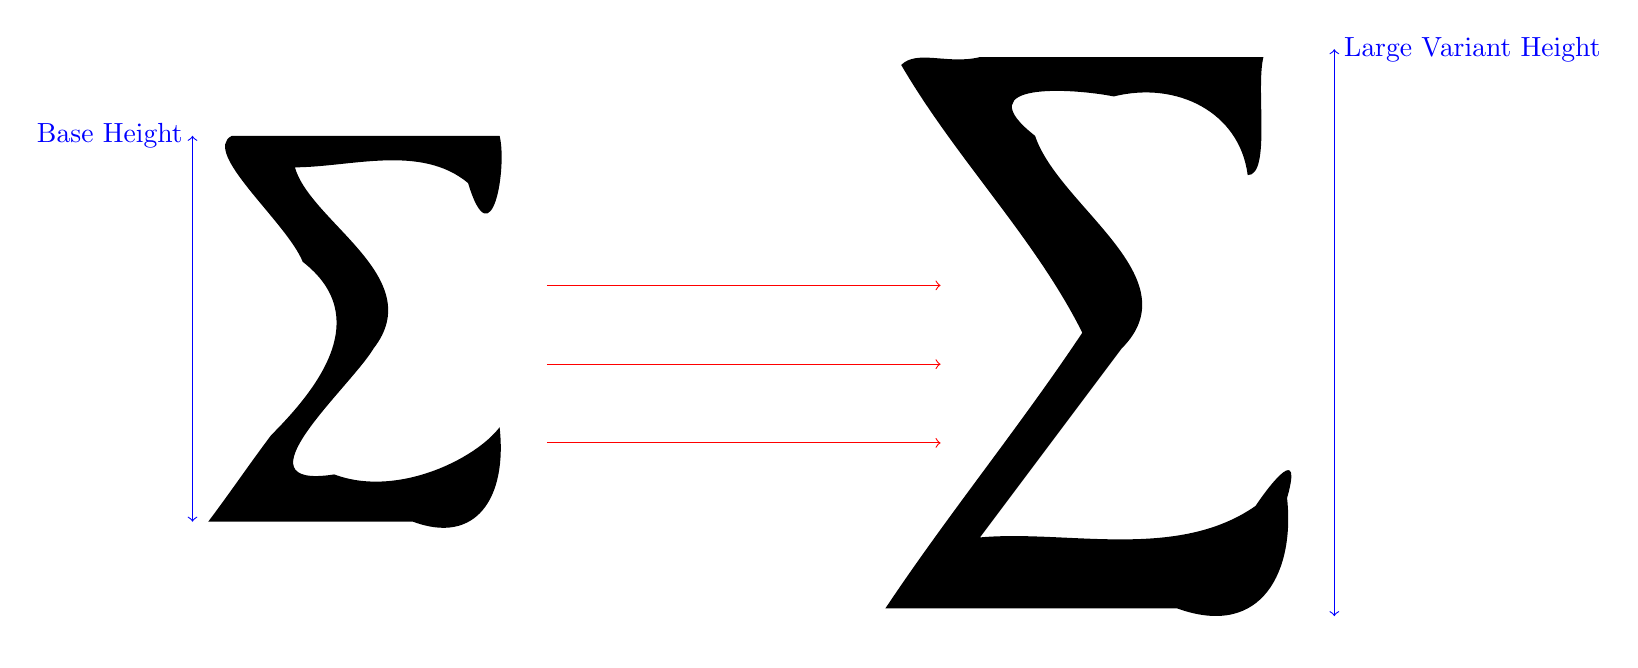
\begin{tikzpicture}[yscale=-1]

    \begin{scope}[xscale=.1,yscale=.1]
    \fill[black](63,71) .. controls (71,59) and (80,48) .. (88,36) .. controls (82,24) and (72,14) .. (65,2) .. controls (67,0) and (71,2) .. (75,1) .. controls (87,1) and (99,1) .. (111,1) .. controls (110,5) and (112,16) .. (109,16) .. controls (108,8) and (100,4) .. (92,6) .. controls (87,5) and (73,4) .. (82,11) .. controls (85,20) and (102,29) .. (93,38) .. controls (87,46) and (81,54) .. (75,62) .. controls (86,61) and (100,65) .. (110,58) .. controls (112,55) and (116,50) .. (114,57) .. controls (115,66) and (111,75) .. (100,71) .. controls (88,71) and (75,71) .. (63,71);
    \draw[blue,<->] (-25,11)node[left]{Base Height} -- (-25, 60);

    \draw[red,->] (20,30) -- (70,30);
    \draw[red,->] (20,40) -- (70,40);
    \draw[red,->] (20,50) -- (70,50);

    \begin{scope}[shift={(-25,0)}]
    \fill[black](10,49) .. controls (16,43) and (23,34) .. (14,27) .. controls (12,22) and (1,13) .. (5,11) .. controls (16,11) and (27,11) .. (39,11) .. controls (40,15) and (38,27) .. (35,17) .. controls (29,12) and (20,15) .. (13,15) .. controls (15,22) and (30,29) .. (23,38) .. controls (20,43) and (5,56) .. (18,54) .. controls (26,57) and (36,52) .. (39,48) .. controls (40,57) and (36,63) .. (28,60) .. controls (19,60) and (10,60) .. (2,60) .. controls (5,56) and (7,53) .. (10,49);
    \draw[blue,<->] (145,0)node[right]{Large Variant Height} -- (145, 72);
    \end{scope}
    \end{scope}
\end{tikzpicture}
\end{document}
